\chapter{Исследовательская часть}

В данном разделе будут приведены примеры работы программы, и будет проведен сравнительный анализ реализованных алгоритмов поиска в словаре по затраченному процессорному времени и по числу сравнений при поиске.

\section{Технические характеристики}

Тестирование проводилось на устройстве со следующими техническими характеристиками:

\begin{itemize}
	\item операционная система: Ubuntu 20.04.1 Linux x86\_64 \cite{linux};
	\item память : 8 GiB;
	\item процессор: AMD® Ryzen™ 3 3200u @ 2.6 GHz \cite{amd}.
\end{itemize}

Тестирование проводилось на ноутбуке, включенном в сеть электропитания. Во время тестирования ноутбук был нагружен только встроенными приложениями окружения, а также непосредственно системой тестирования.

\clearpage

\section{Демонстрация работы программы}

На рисунке \ref{img:example-yes} приведен пример работы программы при наличии введенного ключа в словаре, на рисунке \ref{img:example-no} - при отсутствии введенного ключа в словаре.

\begin{figure}[H]
	\begin{center}
		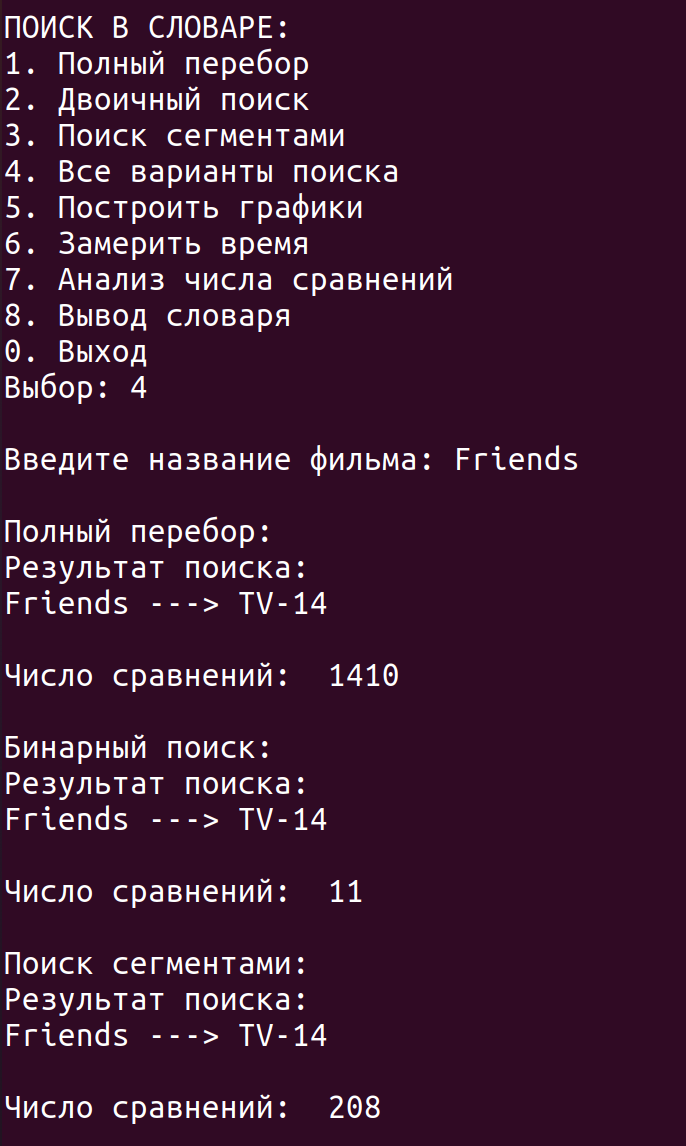
\includegraphics[scale=0.3]{img/example-yes.png}
	\end{center}
	\captionsetup{justification=centering}
	\caption{Пример работы программы (ключ найден)}
	\label{img:example-yes}
\end{figure}

\begin{figure}[H]
	\begin{center}
		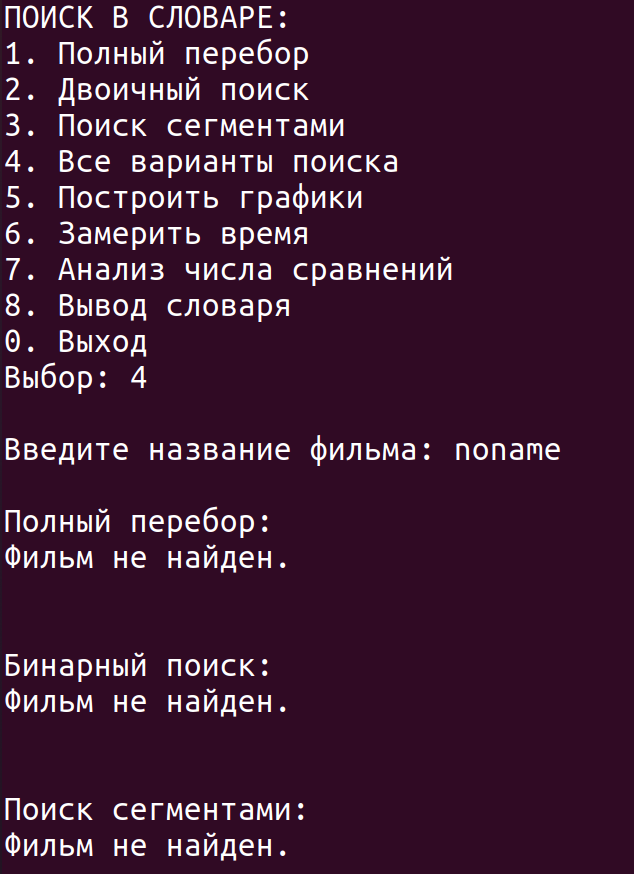
\includegraphics[scale=0.3]{img/example-no.png}
	\end{center}
	\captionsetup{justification=centering}
	\caption{Пример работы программы (ключ не найден)}
	\label{img:example-no}
\end{figure}

\section{Время выполнения алгоритмов}

Функция process\_time из библиотеки time ЯП Python возвращает  процессорное время в секундах - значение типа float.

Для замера времени необходимо получить значение времени до начала выполнения алгоритма, затем после её окончания. Чтобы получить результат, необходимо вычесть из второго значения первое. Замеры проводились 40 раз для получения точного результата.

Замеры проводились для всех ключей словаря. Графическое представление результатов измеренения времени работы алгоритмов приведено на рисунке \ref{img:time}.

\begin{figure}[H]
	\begin{center}
		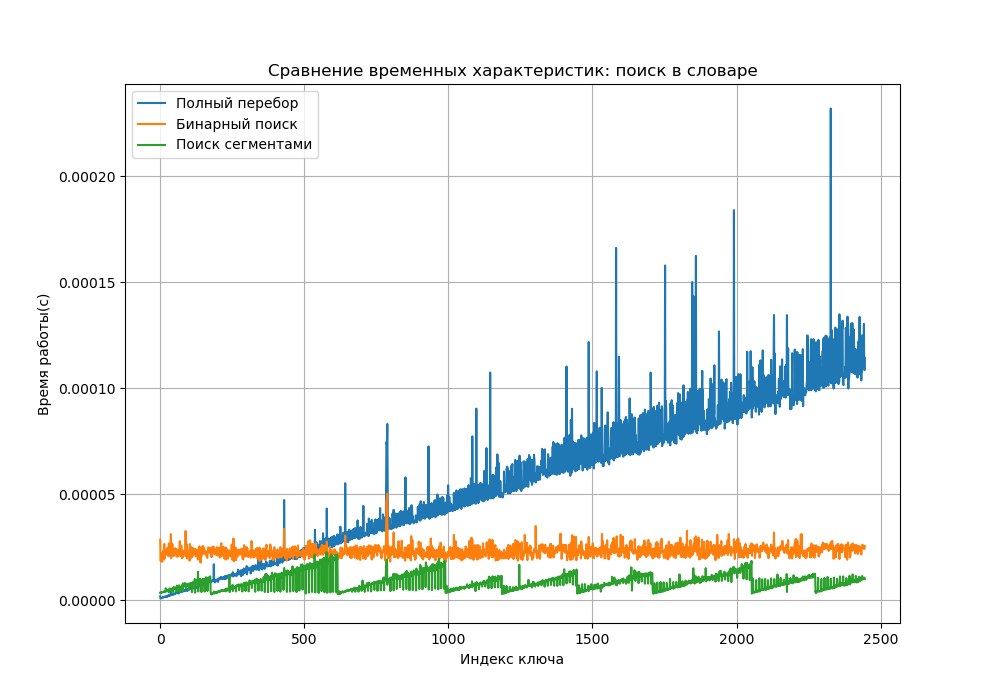
\includegraphics[scale=0.5]{img/time.png}
	\end{center}
	\captionsetup{justification=centering}
	\caption{Сравнительный анализ алгоритмов поиска в словаре по времени}
	\label{img:time}
\end{figure}

\section{Число сравнений при поиске в словаре}

Для всех алгоритмов поиска в словаре был проведен сравнительный анализ по числу сравнений для всех ключей в словаре. Были сопоставлены две гистограммы для каждого из алгоритмов поиска:

\begin{itemize}
	\item ключи расположены в порядке их расположения в словаре;
	\item ключи отсортированы по убыванию числа сравнений.
\end{itemize}

Полученные гистограммы для поиска полным перебором представлены на рисунке \ref{img:brute-cmprs}, для бинарного поиска - на рисунке \ref{img:binary-cmprs}, для поиска сегментами - на рисунке \ref{img:segment-cmprs}.

\begin{figure}[H]
	\begin{center}
		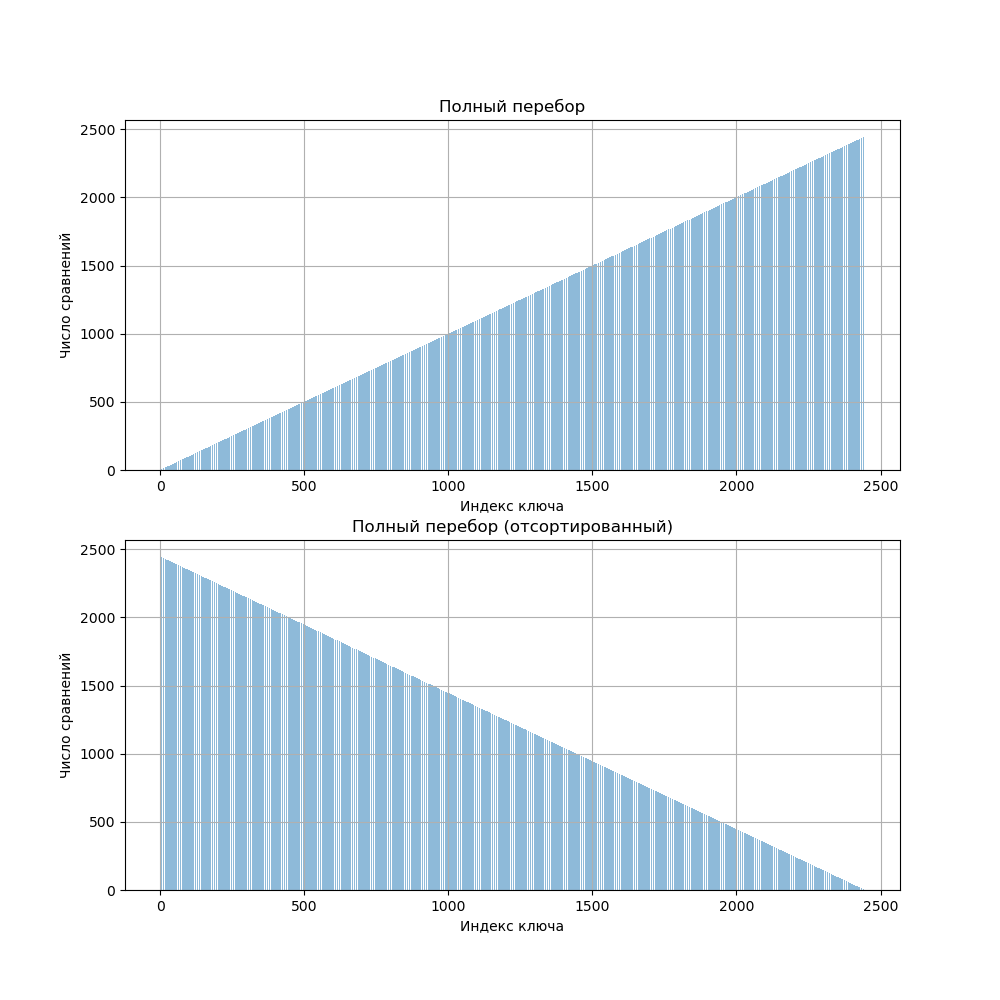
\includegraphics[scale=0.5]{img/brute_cmprs.png}
	\end{center}
	\captionsetup{justification=centering}
	\caption{Сравнительный анализ алгоритмов поиска в словаре по числу сравнений - полный перебор}
	\label{img:brute-cmprs}
\end{figure}

\begin{figure}[H]
	\begin{center}
		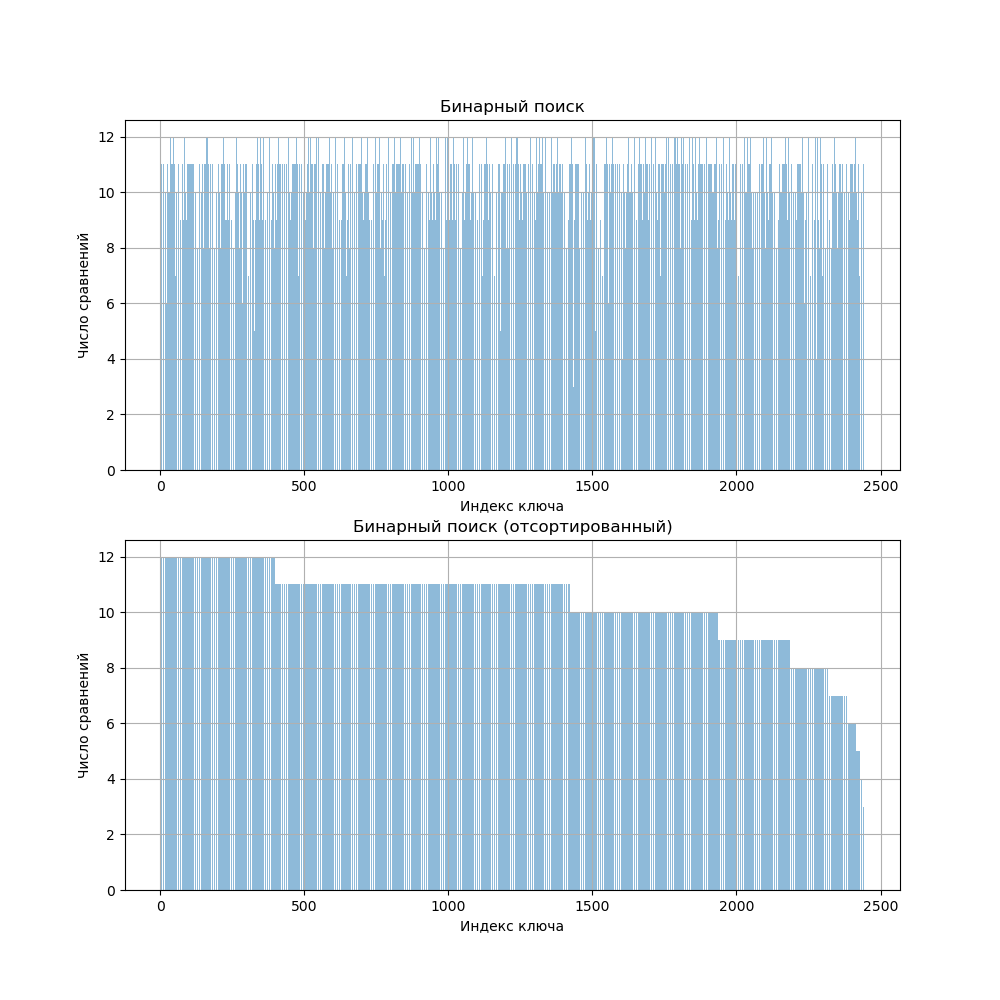
\includegraphics[scale=0.5]{img/binary_cmprs.png}
	\end{center}
	\captionsetup{justification=centering}
	\caption{Сравнительный анализ алгоритмов поиска в словаре по числу сравнений - бинарный поиск}
	\label{img:binary-cmprs}
\end{figure}

\begin{figure}[H]
	\begin{center}
		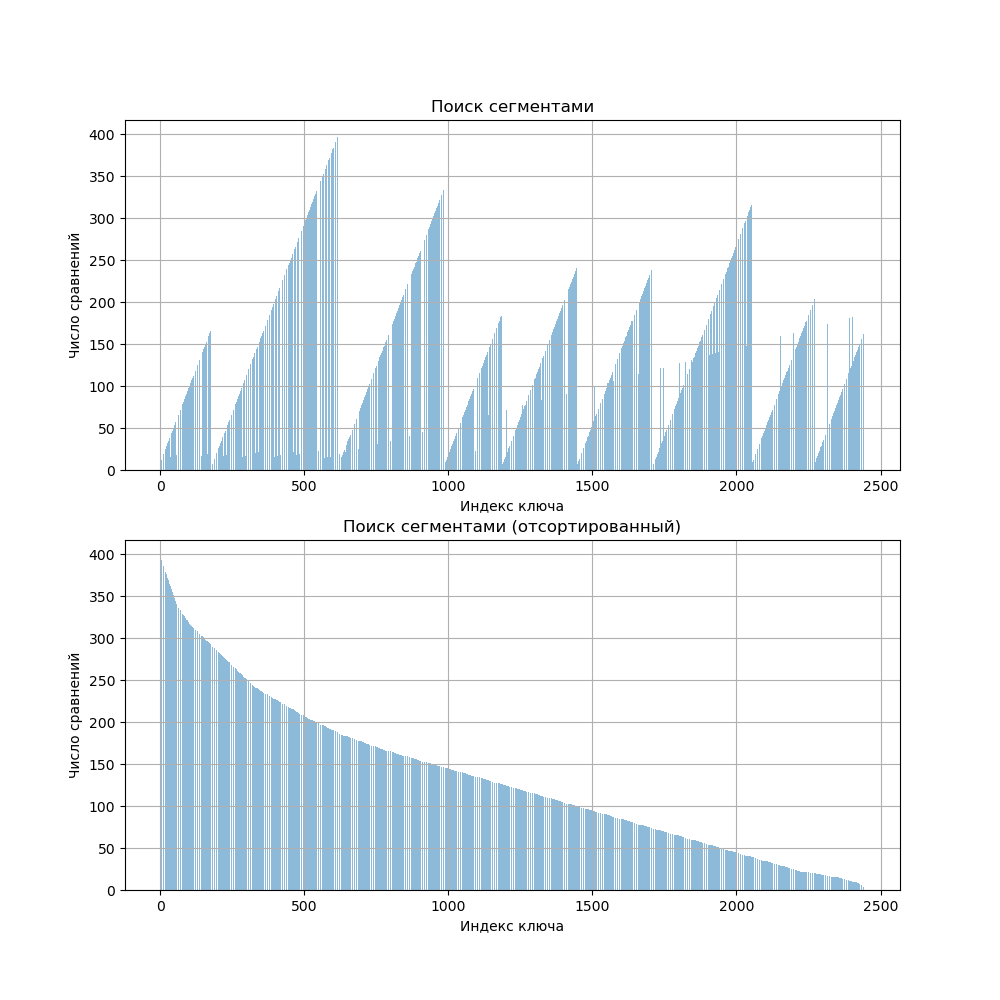
\includegraphics[scale=0.5]{img/segment_cmprs.png}
	\end{center}
	\captionsetup{justification=centering}
	\caption{Сравнительный анализ алгоритмов поиска в словаре по числу сравнений - сегментный поиск}
	\label{img:segment-cmprs}
\end{figure}

\section{Вывод}

В результате эксперимента было получено:
\begin{itemize}
	\item время работы поиска при помощи полного перебора увеличивется пропорционально дальности ключа в словаре;
	\item бинарный и сегментный поиск имеют в среднем одинаковое время поиска всех ключей;
	\item при большом количестве ключей, близком к 2500, сегментный поиск работает быстрее полного перебора в 14 раз, бинарный поиск работает быстрее полного перебора в 6 раз.
\end{itemize}

Можно сделать вывод о том, что при обработке больших данных (близком к 2500) необходимо использовать поиск сегментами.

Также в результате сравнительного анализа было получено, что алгоритму бинарного поиска требуется меньшее число сравнений в сравнении с полным перебором и сегментным поиском. Для поиска в словаре значений, используемом при выполнении данной работы, максимальные числа сравнений:

\begin{itemize}
	\item для бинарного поиска - 12;
	\item для сегментного поиска - 398;
	\item для полного перебора - 2446.
\end{itemize}

Таким образом, в задачах с ограничением по числу сравнений при поиске необходимо использовать бинарный поиск в словаре.